\documentclass{article}
\usepackage{iclr2027_conference,times}

\usepackage[utf8]{inputenc}
\usepackage[T1]{fontenc}
\usepackage[hypertexnames=false]{hyperref}
\hypersetup{colorlinks=true,linkcolor=blue!50!black,citecolor=blue!50!black,urlcolor=blue!50!black}
\usepackage{url}
\usepackage{amsmath,amssymb,amsthm,mathtools}
\usepackage{booktabs}
\usepackage{tabularx}
\usepackage{multirow}
\usepackage{graphicx}
\usepackage{xcolor}
\usepackage{algorithm}
\usepackage{algorithmic}
\usepackage{tikz}
\usetikzlibrary{arrows.meta,positioning,calc,fit,backgrounds}
\usepackage{pgfplots}
\pgfplotsset{compat=1.17}
\usepackage[capitalise,noabbrev]{cleveref}

%% Anonymity switch (restore the public repository at camera-ready)
\newcommand{\anonrepo}{\url{https://anonymous.4open.science/r/SODE-ExtractGuard-Models}}

\newtheorem{theorem}{Theorem}
\renewcommand{\thetheorem}{\Alph{theorem}}
\newtheorem{proposition}{Proposition}
\newtheorem{lemma}{Lemma}
\newtheorem{corollary}{Corollary}
\newtheorem{assumption}{Assumption}
\theoremstyle{definition}
\newtheorem{definition}{Definition}
\newtheorem{remark}{Remark}
\crefname{assumption}{Assumption}{Assumptions}

\newcommand{\Real}{\mathbb{R}}
\newcommand{\Exp}{\mathbb{E}}
\newcommand{\Prob}{\mathbb{P}}
\newcommand{\tr}{\top}
\DeclareMathOperator*{\argmax}{arg\,max}
\newcommand{\ci}[1]{{\scriptsize$\pm$#1}}

\title{Stochastic ODE-Guard: Robust and Certified\\Neural SDE Intrusion Detection}

\author{Anonymous authors\\Paper under double-blind review}

\begin{document}
\maketitle

\begin{abstract}
Neural intrusion detectors summarise every network flow by a few dozen traffic
statistics, and an attacker who controls part of the traffic can shift those
statistics. We present \emph{Stochastic ODE-Guard} (SODE-Guard), a neural
stochastic differential equation (SDE) detector that evolves an encoded flow
under learned random dynamics and classifies by averaging over paths, together
with a training and certification recipe built for it. The recipe has three
modules: imbalance-aware training with a post-hoc logit adjustment; adversarial
training whose adversary differentiates through the deployed multi-path
predictor with fresh Brownian paths; and a randomised-smoothing certificate
that treats Gaussian input noise as a pure-diffusion prefix of the SDE and
samples it jointly with the model's own paths. We prove that this certificate
is sound for the stochastic predictor, and we keep a deterministic Lipschitz
certificate for the discretised SDE. On the container-flow part of the ICS3D
benchmark, deduplicated and evaluated over five seeds against eight adaptive
attacks, the recipe raises clean macro-F1 from $0.438$ to $0.495$, worst-case
macro-F1 from $0.245$ to $0.420$, and certified accuracy at $\ell_2$ radius
$0.273$ to $0.576$ ($0.877$ on the test class mix), on par with the strongest
adversarially trained and smoothed baselines. Gradient-boosted trees, the most
accurate clean models, fall to $0.02$ under a black-box attack and to $0.17$
when the attacker may change only realisable traffic statistics, a setting in
which SODE-Guard keeps $0.446$; conformal alarm thresholds hold its false-alarm
rate at the chosen budget. On UNSW-NB15, a second corpus from a different
network and feature extractor, every conclusion carries over, and SODE-Guard is
significantly ahead of the matched MLP both under attack and in certified
accuracy.
SODE-Guard gives security teams a detector whose robustness is measured under
adaptive attack and certified by its own randomness, and gives researchers an
open, reproducible protocol for building and testing robust intrusion detectors.
\end{abstract}

%% ==================================================================
\section{Introduction}\label{sec:intro}
%% ==================================================================
Network intrusion detection and prevention systems (IDPS) decide, flow by flow,
whether traffic is benign or belongs to an attack. A \emph{flow} is the set of
packets exchanged between two endpoints in one session, and modern detectors
summarise it by statistics such as duration, packet and byte counts,
inter-arrival times and protocol flags. Learned detectors on such summaries now
cover enterprise, cloud and industrial networks
\citep{lo2022egraphsage,wu2022rtids,anaedevha2026mstgnn}.
They are also exposed: an attacker who pads packets or adds delays controls
some of the statistics, and small, deliberately chosen changes remove many F1
points from standard detectors \citep{ennaji2024advsurvey,vitorino2024advbench,anaedevha2024robust}.

A deployable robust detector has to satisfy three requirements at once. It must
learn the rare attack classes, not only the frequent ones; it must keep its
accuracy against an attacker who adapts to the model, including its
randomness \citep{athalye2018obfuscated,carlini2019evaluating}; and it should
come with a guarantee that holds for every admissible change, a
\emph{certificate}. Continuous-time models are a natural candidate. Neural ODEs
inherit stability from their flow map \citep{kang2021sodef}, and neural SDEs
\citep{tzen2019nsde,li2020scalable} add learned noise that is well posed and
carries calibrated uncertainty \citep{oh2024stablesde,liu2020sdenoise}.
Stochastic and continuous-time intrusion detectors
\citep{anaedevha2026ode,anaedevha2026mstgnn} already deliver
strong clean accuracy and uncertainty estimates; this paper turns such a model
into a detector that is trained, attacked and certified under one protocol.

\paragraph{This paper.} SODE-Guard encodes a flow into a 128-dimensional state,
evolves the state under a learned SDE and classifies by averaging a linear
read-out over eight random paths (\cref{fig:arch}). Around this model we build
a recipe of three modules and a measurement protocol strict enough for
security use.

\paragraph{Contributions.}
\textbf{(C1) A sound certificate that uses the model's own noise.} We show that
Gaussian input noise is a pure-diffusion prefix of the SDE and that randomised
smoothing remains sound when the base classifier is itself random
(\cref{prop:smooth}). SODE-Guard is therefore certified by sampling input noise
and Brownian paths jointly, with no separate noisy copy of the model. A
deterministic Lipschitz certificate for the Euler--Maruyama scheme
(\cref{thm:mean-cert}) complements it.
\textbf{(C2) A training recipe for stochastic detectors.} Imbalance-aware
training with a post-hoc logit adjustment raises clean macro-F1 by $0.057$;
adversarial training through the deployed multi-path predictor raises
worst-case macro-F1 by $0.174$; longer smoothing-aware training raises
certified accuracy by $0.020$ (all significant over five seeds, Holm-corrected).
\textbf{(C3) A protocol a security reviewer can trust.} Deduplication before
splitting, five seeds with new splits, eight adaptive attacks scored with
fixed and fresh paths, gradient-masking checks, a full-strength re-attack,
feature-constrained attacks, a per-class chronological split, tree baselines,
conformal operating points and paired-bootstrap contrasts declared before the
runs.
\textbf{(C4) Findings that guide deployment, on two corpora.} With the recipe,
SODE-Guard is never worse than the strongest adversarially trained and smoothed
baselines and pulls ahead of them on UNSW-NB15, and
gradient-boosted trees, the best clean models, collapse under attack, also when
the attacker is limited to realisable changes, so robust neural detectors are
needed exactly where trees look best.
Code, configurations and every result file are in an anonymised repository
(\anonrepo).

%% ==================================================================
\section{Setting and background}\label{sec:setting}
%% ==================================================================
This section fixes the problem, the attacker and the two notions of
guarantee we use; \cref{tab:notation} collects the notation.

\begin{table}[t]
\caption{Notation.}
\label{tab:notation}
\centering\footnotesize
\renewcommand{\arraystretch}{1.1}
\begin{tabularx}{\linewidth}{@{}l>{\raggedright\arraybackslash}X@{\hspace{6pt}}l>{\raggedright\arraybackslash}X@{}}
\toprule
Symbol & Meaning & Symbol & Meaning\\
\midrule
$x\in\Real^{p}$ & flow statistics, $p=75$, z-scored & $K$, $\pi$ & number of classes ($9$), training class prior\\
$\delta$, $\varepsilon$ & perturbation, $\ell_\infty$ budget ($0.03$) & $\|\cdot\|_2$, $\|\cdot\|_\infty$ & Euclidean, max-coordinate norm\\
$h$, $X_0=h(x)$ & encoder, initial state in $\Real^{d}$, $d=128$ & $W_t$ & Brownian motion in $\Real^{m}$, $m=16$\\
$f_\theta$, $g_\theta$ & drift, diffusion of the SDE & $T$, $\Delta t$, $n$ & horizon $1$, step $0.05$, $20$ steps\\
$M$, $F_M(x)$ & paths at inference ($8$), mean logits & $b$, $\tau'$ & post-hoc bias $b=-\tau'\log\pi$\\
$\sigma$, $\lambda$ & smoothing noise ($0.25$), consistency weight & $G(x)$, $p_c(x)$ & smoothed classifier, class probability\\
$L$ & Lipschitz constant of the mean logits & $r(x)$ & certified $\ell_2$ radius\\
$n_0$, $n$ & selection and estimation draws & $\alpha$ & failure probability of a certificate\\
\bottomrule
\end{tabularx}
\end{table}

\textbf{Flows and metrics.} A flow is described by $p=75$ numeric statistics,
each \emph{z-scored} with training statistics, so one unit is one standard
deviation. A detector outputs $K$ scores (\emph{logits}), and the predicted
class is the largest. Attack classes are highly imbalanced, so we report
\emph{macro-F1}, $\frac1K\sum_k 2P_kR_k/(P_k+R_k)$ with precision $P_k$ and
recall $R_k$ of class $k$, which weighs a rare attack as much as the benign
class, next to accuracy.

\textbf{Threat model and adaptive attacks.} The adversary replaces $x$ by
$x+\delta$ with $\|\delta\|_\infty\le\varepsilon=0.03$, three hundredths of a
standard deviation per statistic, and knows the model, its weights and its
noise distribution (white box). Since $\|\delta\|_2\le\sqrt{p}\,\|\delta\|_\infty$,
this budget lies inside the $\ell_2$ ball of radius $0.03\sqrt{75}=0.26$; we
report certificates at the slightly larger radius $0.273$. Against a randomised
model the attacker averages gradients over the randomness (expectation over
transformation, EOT, \citealp{athalye2018obfuscated}). The \emph{worst case}
counts a flow as misclassified if any attack in a suite succeeds on it, and
macro-F1 is computed on these per-flow worst outcomes. \emph{Adversarial
training} \citep{madry2018pgd} fits the model on attacked inputs,
$\min_\theta\Exp_{(x,y)}\max_{\|\delta\|\le\varepsilon}\ell(F(x+\delta),y)$, with
the inner maximum approximated by an attack.

\textbf{Certified robustness.} Attacks show that some attacker failed; a
certificate proves that every attacker within a budget fails.

\begin{definition}[Certified radius and certified accuracy]\label{def:cert}
A number $r(x)\ge0$ is a \emph{certified $\ell_2$ radius} of a classifier at $x$
if its decision is the same for every $x+\delta$ with $\|\delta\|_2\le r(x)$. The
\emph{certified accuracy} at radius $r$ is the fraction of test flows that are
classified correctly with radius at least $r$; abstentions count as errors.
\end{definition}

Two routes give certificates. A \emph{Lipschitz} certificate uses a bound $L$
on how fast the logits can change, $\|F(x)-F(x')\|_2\le L\|x-x'\|_2$; a gap $M(x)$
between the top two logits then cannot close within radius $M(x)/(\sqrt2L)$
\citep{tsuzuku2018lipschitz}. \emph{Randomised smoothing}
\citep{cohen2019smoothing} classifies by the most likely decision under Gaussian
input noise, $G(x)=\argmax_c\Prob[f(x+\sigma\epsilon)=c]$; if the top class has
probability at least $\underline p_A>\tfrac12$, $G$ is constant within radius
$\sigma\Phi^{-1}(\underline p_A)$, whatever the base classifier $f$.

\textbf{Neural SDEs.} An It\^o SDE
$dX_t=f_\theta(X_t,t)\,dt+g_\theta(X_t,t)\,dW_t$ moves a state $X_t\in\Real^d$
along a learned \emph{drift} $f_\theta$ and adds Gaussian noise shaped by a
learned \emph{diffusion} $g_\theta\in\Real^{d\times m}$, driven by a Brownian
motion $W_t\in\Real^m$, whose increments over a step $\Delta t$ are independent
$\mathcal N(0,\Delta t\,I_m)$ vectors. On a computer it is solved by the
Euler--Maruyama (EM) scheme
\begin{equation}\label{eq:em}
  X_{k+1}=X_k+f_\theta(X_k,t_k)\,\Delta t+g_\theta(X_k,t_k)\,\Delta W_k,\qquad
  \Delta W_k\sim\mathcal N(0,\Delta t\,I_m),
\end{equation}
and one run of \eqref{eq:em} with one draw of the increments is a \emph{path}.
All our statements concern \eqref{eq:em}, the scheme that is actually run.

%% ==================================================================
%% ==================================================================
\section{Related work}\label{sec:related}
%% ==================================================================
\textbf{Robust and certified classifiers.} Adversarial training
\citep{madry2018pgd,zhang2019trades} remains the most reliable empirical
defence; single-step variants with noise \citep{dejorge2022nfgsm} make it
cheap, and early stopping on robust validation accuracy prevents robust
overfitting \citep{rice2020overfitting}. Lipschitz-bounded networks
\citep{tsuzuku2018lipschitz,anil2019sorting,araujo2023sll} certify radii that
scale with the inverse Lipschitz constant. Randomised smoothing
\citep{cohen2019smoothing,salman2019smoothadv,yang2020smoothing} certifies
majority votes over Gaussian noise; consistency regularisation
\citep{jeong2020consistency} improves it, and BARS \citep{wang2023bars} and
MARS \citep{huang2025mars} adapt the noise to traffic features. Adaptive
evaluation needs EOT, attack ensembles and masking checks
\citep{athalye2018obfuscated,croce2020autoattack,carlini2019evaluating}.

\textbf{Neural ODEs and SDEs.} SODEF \citep{kang2021sodef} uses Lyapunov-stable
equilibria; stable neural SDEs \citep{oh2024stablesde} and latent graph neural
SDEs \citep{bergna2024lgnsde} establish well-posedness;
\citet{liu2020sdenoise} explain noise injection through the neural SDE lens. We
add a certificate that draws on the SDE's own noise and a training recipe tested
against adaptive attacks.

\textbf{Intrusion detection.} Graph \citep{lo2022egraphsage}, transformer
\citep{wu2022rtids}, recurrent \citep{halbouni2022cnnlstm} and state-space
\citep{mosaiyebzadeh2025graphmamba} detectors model flows and their context.
Continuous-time and stochastic detectors
\citep{anaedevha2026ode,anaedevha2026mstgnn} and uncertainty-aware models with
stochastic and PAC-Bayesian formulations
\citep{anaedevha2025stochtx,anaedevha2026pacbayes} supply calibrated scores, and
adversarial training improves the robustness of flow classifiers to evasion
\citep{anaedevha2024robust}.
\citet{arp2022dos}, \citet{pendlebury2019tesseract} and
\citet{engelen2021troubleshooting} show how leakage, sampling bias and label
errors inflate security-ML results, and \citet{grinsztajn2022trees} show that
tree ensembles remain strong on tabular data; our protocol builds on both
lessons, and \citet{simonetto2024tabularbench} benchmark tabular robustness
under feature constraints.

%% ==================================================================
\section{SODE-Guard and its training recipe}\label{sec:model}
%% ==================================================================
\begin{figure}[t]
\centering
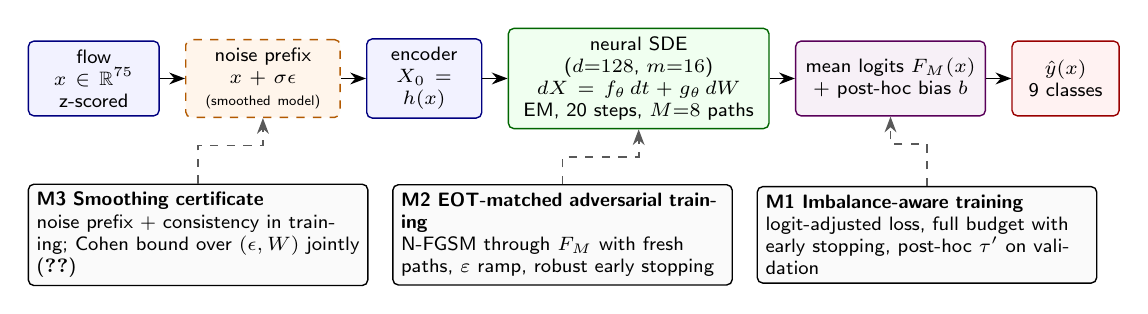
\begin{tikzpicture}[
  font=\sffamily\scriptsize, >=Stealth,
  box/.style={draw, rounded corners=2pt, align=center, minimum height=0.95cm, inner sep=3pt, line width=0.5pt},
  mod/.style={draw, rounded corners=2pt, align=left, inner sep=3pt, text width=4.1cm, line width=0.5pt},
  arr/.style={->, line width=0.6pt}]
\node[box, fill=blue!5, draw=blue!50!black, text width=1.45cm] (x) {flow $x\in\Real^{75}$\\z-scored};
\node[box, fill=orange!8, draw=orange!70!black, dashed, text width=1.75cm, right=0.32cm of x] (pre)
  {noise prefix\\$x+\sigma\epsilon$\\{\tiny (smoothed model)}};
\node[box, fill=blue!5, draw=blue!50!black, text width=1.25cm, right=0.32cm of pre] (h) {encoder\\$X_0=h(x)$};
\node[box, fill=green!6, draw=green!40!black, text width=3.1cm, right=0.32cm of h] (sde)
  {neural SDE ($d{=}128$, $m{=}16$)\\$dX=f_\theta\,dt+g_\theta\,dW$\\EM, 20 steps, $M{=}8$ paths};
\node[box, fill=violet!6, draw=violet!70!black, text width=2.2cm, right=0.32cm of sde] (head)
  {mean logits $F_M(x)$\\$+$ post-hoc bias $b$};
\node[box, fill=red!5, draw=red!60!black, text width=1.15cm, right=0.32cm of head] (y) {$\hat y(x)$\\9 classes};
\draw[arr] (x)--(pre); \draw[arr] (pre)--(h); \draw[arr] (h)--(sde); \draw[arr] (sde)--(head); \draw[arr] (head)--(y);
\node[mod, fill=gray!4, below=0.85cm of x.south west, anchor=north west] (m3)
  {\textbf{M3 Smoothing certificate}\\noise prefix + consistency in training; Cohen bound over $(\epsilon,W)$ jointly (\cref{prop:smooth})};
\node[mod, fill=gray!4, right=0.3cm of m3] (m2)
  {\textbf{M2 EOT-matched adversarial training}\\N-FGSM through $F_M$ with fresh paths, $\varepsilon$ ramp, robust early stopping};
\node[mod, fill=gray!4, right=0.3cm of m2] (m1)
  {\textbf{M1 Imbalance-aware training}\\logit-adjusted loss, full budget with early stopping, post-hoc $\tau'$ on validation};
\draw[arr, dashed, gray!70!black] (m3.north) |- ([yshift=-0.35cm]pre.south) -- (pre.south);
\draw[arr, dashed, gray!70!black] (m2.north) |- ([yshift=-0.35cm]sde.south) -- (sde.south);
\draw[arr, dashed, gray!70!black] (m1.north) |- ([yshift=-0.35cm]head.south) -- (head.south);
\end{tikzpicture}
\caption{SODE-Guard. Solid arrows: inference. A flow is encoded, evolved by the
learned SDE over $M=8$ random paths, read out linearly and averaged; a post-hoc
bias tuned on validation data completes the deployed predictor. The noise
prefix (dashed box) is active only in the smoothed variant. Dashed arrows: the
three modules of the recipe and the part of the model each one acts on.}
\label{fig:arch}
\end{figure}

\textbf{Model.} The encoder $h$ maps $x$ to $X_0\in\Real^{128}$; the SDE has
$m=16$ noise channels, three-layer drift and diffusion networks of width 256
with spectral normalisation and a diffusion floor $\lambda_0=10^{-3}$, horizon
$T=1$ and $\Delta t=0.05$. A linear head $\psi$ gives $K$ logits, and the
deployed predictor is
\begin{equation}\label{eq:predictor}
  F_M(x)=\frac1M\sum_{j=1}^{M}\psi\bigl(X_n^{(j)}\bigr)+b,\qquad
  \hat y(x)=\argmax_k F_{M,k}(x),
\end{equation}
the mean logits of $M=8$ paths started at $h(x)$, plus a bias $b$ fixed after
training (M1). Its population version $F(x)=\Exp[\psi(X_n)]+b$ is the object of
\cref{thm:mean-cert}. The three modules below are what make this model a
robust detector.

\textbf{M1: imbalance-aware training.} Rare attacks dominate macro-F1. We train
with the logit-adjusted loss \citep{menon2021logit}
$\ell(F_M(x)+\tau\log\pi,\,y)$, where $\pi$ is the training class prior and
$\ell$ the cross-entropy, with AdamW, cosine decay and up to 60 epochs, keeping
the epoch with the best macro-F1 on a \emph{selection} half of the validation
split. After training, the bias $b=-\tau'\log\pi$ is tuned on the same half
(post-hoc logit adjustment). The other validation half is held out for
calibration.

\textbf{M2: EOT-matched adversarial training.} The training adversary attacks
exactly the predictor \eqref{eq:predictor}, with fresh Brownian paths at every
step, so the model cannot hide behind its own randomness. We use N-FGSM
\citep{dejorge2022nfgsm}: $\tilde x=x+\eta+\varepsilon\,\mathrm{sign}\,\nabla_x
\ell(F_M(x+\eta),y)$ with $\eta\sim\mathcal U[-2\varepsilon,2\varepsilon]^p$, at
about twice the cost of a clean step. The budget ramps up over the first 15\%
of epochs, and the kept epoch maximises macro-F1 under PGD-10 on validation
flows \citep{rice2020overfitting}.

\textbf{M3: smoothing-aware training and certificate.} For the smoothed
variant, the input first passes a pure-diffusion prefix: integrating
$dZ_s=\sigma\,dB_s$ for unit time from $Z_0=x$ gives $Z_1=x+\sigma\epsilon$,
$\epsilon\sim\mathcal N(0,I_p)$, after which the learned SDE runs as before. We
train on two noisy copies per flow with consistency regularisation
\citep{jeong2020consistency}, the loss
$\tfrac12\sum_i\ell(F_M(x+\sigma\epsilon_i),y)
+\lambda\,\tfrac12\sum_i\mathrm{KL}(\bar p\,\|\,p_i)+\eta_{\mathrm H}H(\bar p)$, where
$p_i$ is the softmax of copy $i$ and $\bar p$ their mean. We use $\sigma=0.25$
and train for at least 20 epochs, selecting on the noisy-vote macro-F1 after
the post-hoc adjustment. \Cref{sec:theory} shows how the certificate follows.

%% ==================================================================
\section{Guarantees}\label{sec:theory}
%% ==================================================================
\textbf{A smoothing certificate for a stochastic detector.} Let
$\hat y(z;\omega)$ denote the deployed decision at input $z$ when the Brownian
paths are $\omega$, drawn independently of $z$. The smoothed SODE-Guard is
\begin{equation}\label{eq:smoothed}
  G(x)=\argmax_c\;p_c(x),\qquad p_c(x)=\Prob_{\epsilon,\omega}\bigl[\hat y(x+\sigma\epsilon;\omega)=c\bigr],
\end{equation}
the most likely decision of the model fed through the noise prefix.

\begin{proposition}[Smoothing certificate for a random base classifier]\label{prop:smooth}
Let $\epsilon\sim\mathcal N(0,I_p)$ and $\omega$ be independent of each other
and of $x$, and suppose $p_{c_A}(x)\ge\underline p_A>\tfrac12$. Then
$G(x+\delta)=c_A$ for every $\|\delta\|_2<\sigma\,\Phi^{-1}(\underline p_A)$,
where $\Phi$ is the standard normal distribution function. If
$\underline p_A$ is the one-sided Clopper--Pearson lower bound at level
$1-\alpha$ from $n$ independent draws of $(\epsilon,\omega)$, the statement holds
with probability at least $1-\alpha$.
\end{proposition}

\emph{Why it holds.} Averaging over the paths first turns the random detector
into a soft one, $u_c(z)=\Prob_\omega[\hat y(z;\omega)=c]\in[0,1]$, and
$p_c=u_c*\mathcal N(0,\sigma^2I)$. For any $[0,1]$-valued function, the
Gaussian convolution satisfies that $x\mapsto\sigma\Phi^{-1}(p_c(x))$ is
1-Lipschitz \citep[Lemma~2]{salman2019smoothadv}, so $p_{c_A}$ stays above
$\tfrac12$, and every other class below it, inside the stated radius. Joint
draws of $(\epsilon,\omega)$ are independent Bernoulli trials with success
probability $p_{c_A}(x)$, which makes the Clopper--Pearson bound exact
(\cref{app:proofs}). The certificate therefore needs no noise-free copy of the
model: the paths the detector already samples are part of the smoothing
distribution. We certify with $n_0=100$ selection draws, $n=2000$ estimation
draws and $\alpha=10^{-3}$ (\cref{alg:certify}); the largest radius this $n$ can
certify is $0.675$.




\textbf{A deterministic certificate for the discretised SDE.} The second
guarantee covers every perturbation at once, without input noise. Run the scheme
\eqref{eq:em} from $h(x)$ and from $h(x+\delta)$ with the \emph{same} increments
(synchronous coupling). In one step the drift stretches the gap between the two
paths by at most $1+K_f\Delta t$ and the diffusion adds variance $K_g^2\Delta t$
times the squared gap, which gives:

\begin{lemma}[Mean-square stability]\label{lem:ms}
If $h$, $f_\theta$ and $g_\theta$ are $L_h$-, $K_f$- and $K_g$-Lipschitz in the
state, then $\Exp\|Y_n-X_n\|^2\le L_h^2\|\delta\|^2\exp\bigl((2K_f+K_g^2+K_f^2\Delta t)T\bigr)$.
\end{lemma}

\begin{theorem}[Certified radius of the SDE-mean classifier]\label{thm:mean-cert}
Let $P_B$ project a logit vector onto the ball of radius $B$ and
$F^B(x)=\Exp[P_B(\psi(X_n))]$. With
$L=\|W_\psi\|L_h\exp\bigl((K_f+\tfrac12K_g^2+\tfrac12K_f^2\Delta t)T\bigr)$,
$\|F^B(x+\delta)-F^B(x)\|_2\le L\|\delta\|_2$, and a margin
$M(x)=F^B_{\hat y}(x)-\max_{k\ne\hat y}F^B_k(x)$ certifies the $\ell_2$ radius
$M(x)/(\sqrt2L)$.
\end{theorem}

A Monte-Carlo version with empirical-Bernstein confidence widths turns the
theorem into a procedure that returns a radius or abstains (\cref{cor:mc}), and
a path-wise bound limits the probability that a single path flips its decision
(\cref{prop:flip}); both are proved in \cref{app:proofs}. With spectral
normalisation the constant is computable from the trained weights, and on an
earlier, certifiable configuration of the model the theorem gave non-vacuous
radii on trained detectors (\cref{tab:det-cert}). The smoothing certificate is
our headline guarantee because its radius does not depend on the growth factor
$\exp((K_f+\frac12K_g^2)T)$; the two certificates are complementary, one
probabilistic and tight, the other deterministic and noise-free.

%% ==================================================================
\section{Experiments}\label{sec:exp}
%% ==================================================================
\textbf{Data.} We use the container-flow part of ICS3D \citep{anon_ics3d}, the
Kubernetes misuse-detection flows of \citet{amin2024misuse}, capped at
$20{,}000$ flows per class. Before
any split we drop identifiers and the client-assigned source port, remove 325
exact duplicates and 1{,}250 flows whose features also occur with a different
label, and keep the classes with at least 100 flows: $68{,}627$ flows, 9 classes
(four large classes of $8{,}696$--$19{,}878$ flows and five small ones of
128--803 flows), 75 features. The classes are benign traffic and eight attack
scenarios: four CVE exploits, the reconnaissance, remote-code-execution and
container-escape stages of a Node-RED attack, and a Nuclei scan; three CVE
scenarios with fewer than 100 flows are excluded. As a second corpus we use
UNSW-NB15 \citep{moustafa2015unsw} from the IIS3D collection \citep{anon_iis3d}:
39 numeric features of a different extractor, Normal traffic and nine attack
families, capped at 5{,}000 flows per class. Deduplication removes 4{,}405 exact
duplicates and 11{,}212 flows whose features occur with different attack labels,
a known property of this corpus, which leaves 21{,}074 flows; scores are
therefore not comparable to published results on the uncleaned set. Each of
five seeds draws a new stratified
60/20/20 split (\cref{app:data}).

\textbf{Models and baselines.} SODE-Guard with M1 (\texttt{SODE}), with M1 and
M2 (\texttt{SODE-AT}) and with M1 and M3 (\texttt{SODE-RS}); the same recipe on
a neural ODE (SODE-Guard with $g_\theta=0$) and on an E-GraphSAGE-style MLP
\citep{lo2022egraphsage}; LightGBM \citep{ke2017lightgbm}, XGBoost
\citep{chen2016xgboost} and a random forest \citep{breiman2001rf} with balanced
weights and the same post-hoc adjustment; and the original training recipe
(cross-entropy with the anti-concentration regulariser, 10 epochs, no early
stopping or post-hoc adjustment) as \texttt{SODE-base}.

\textbf{Attacks and statistics.} $\ell_\infty$, $\varepsilon=0.03$, on 500
class-stratified test flows per seed: PGD-40; PGD-100 with two restarts;
APGD-CE and APGD-DLR \citep{croce2020autoattack} with EOT; EOT-PGD-50 with eight
draws; an expected-margin attack on 64 fresh paths per step; Square
\citep{andriushchenko2020square} with 1{,}000 queries; and transfer from two
surrogates. Gradient attacks differentiate through \eqref{eq:predictor}, bias
included. Each adversarial flow is scored with fixed paths (seeds 0--7, a
deterministic target) and with fresh paths, and we report the per-flow worst
case over all attacks. Trees are not differentiable and face Square and
transfer. Results are means over five seeds with 95\% $t$-intervals; every
contrast is a paired bootstrap over flows within seeds, Holm-corrected
\citep{holm1979} over a family declared before the runs.

\begin{table}[t]
\caption{Clean and worst-case macro-F1 over eight adaptive attacks
($\ell_\infty$, $\varepsilon=0.03$); mean $\pm$ 95\% CI over five seeds.
\emph{Fixed}/\emph{fresh}: scored with fixed or fresh Brownian paths. Trees
face the black-box and transfer attacks only.}
\label{tab:main}
\centering\footnotesize
\setlength{\tabcolsep}{3.5pt}
\begin{tabular}{llcccc}
\toprule
& Model & Clean macro-F1 & Clean acc. & Worst case, fixed & Worst case, fresh\\
\midrule
\multirow{4}{*}{\shortstack[l]{standard\\train.}}
& SODE-base (orig.\ recipe) & 0.438\ci{.006} & 0.934\ci{.002} & 0.223\ci{.014} & 0.224\ci{.013}\\
& SODE (M1) & 0.495\ci{.009} & 0.935\ci{.006} & 0.245\ci{.017} & 0.244\ci{.018}\\
& Neural ODE (M1) & 0.490\ci{.003} & 0.931\ci{.005} & 0.243\ci{.019} & ---\\
& MLP (M1) & 0.479\ci{.026} & 0.919\ci{.024} & 0.267\ci{.012} & ---\\
\midrule
\multirow{3}{*}{\shortstack[l]{adv.\\train.}}
& SODE-AT (M1+M2) & 0.468\ci{.013} & 0.918\ci{.011} & \textbf{0.420}\ci{.010} & \textbf{0.412}\ci{.012}\\
& Neural ODE-AT & 0.465\ci{.006} & 0.915\ci{.020} & 0.432\ci{.028} & ---\\
& MLP-AT & 0.462\ci{.019} & 0.915\ci{.017} & 0.424\ci{.047} & ---\\
\midrule
\multirow{3}{*}{trees}
& LightGBM & 0.619\ci{.034} & 0.953\ci{.003} & 0.021\ci{.008} & ---\\
& XGBoost & 0.621\ci{.010} & 0.956\ci{.002} & 0.015\ci{.006} & ---\\
& Random forest & 0.607\ci{.028} & 0.955\ci{.003} & 0.037\ci{.016} & ---\\
\bottomrule
\end{tabular}
\end{table}

\subsection{Clean and adversarial performance}
\textbf{M1 lifts every detector's rare-class performance.} The recipe raises
SODE-Guard's clean macro-F1 from $0.438$ to $0.495$ ($+0.057$,
$p_{\mathrm{Holm}}=0.016$; \cref{tab:main}) at unchanged accuracy; both models share
architecture, data and seeds, so the gain is the module's. With M1, SODE-Guard is above the MLP ($+0.016$,
$p_{\mathrm{Holm}}=0.016$) and level with the neural ODE ($+0.005$).

\textbf{M2 closes the robustness gap.} Adversarial training through the
multi-path predictor raises the worst case from $0.245$ to $0.420$ ($+0.174$,
$p_{\mathrm{Holm}}=0.016$) for $0.027$ of clean macro-F1. SODE-AT matches the
adversarially trained MLP ($-0.001$, CI $[-0.010,0.007]$) and neural ODE
($-0.005$), and fixed and fresh paths agree ($0.420$ vs.\ $0.412$), so the
robustness does not rest on hidden randomness. The eight attacks land within
$0.42$--$0.45$ of each other (\cref{tab:attacks}).

\textbf{Trees are accurate and brittle.} Gradient-boosted trees reach the best
clean macro-F1 ($0.62$), $0.12$ above SODE-Guard, mostly on three mid-sized
attack classes (\cref{tab:perclass}). A 1{,}000-query black-box attack, which
needs no gradients, drives them to $0.015$--$0.037$, while every adversarially
trained neural detector keeps $0.42$--$0.43$ (\cref{fig:results}a). For a
deployment that must withstand evasion, the robust neural detector is the safe
choice.

\begin{figure}[t]
\centering
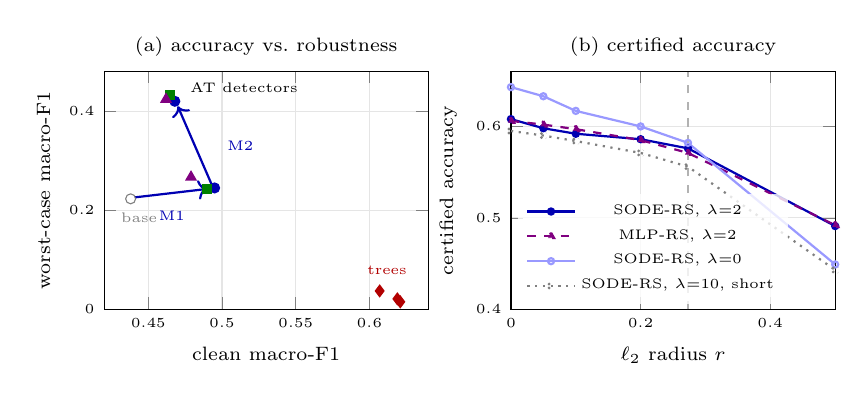
\begin{tikzpicture}
\begin{axis}[
  name=left, width=0.47\linewidth, height=4.6cm,
  xlabel={clean macro-F1}, ylabel={worst-case macro-F1},
  xmin=0.42, xmax=0.64, ymin=0, ymax=0.48,
  label style={font=\scriptsize}, tick label style={font=\tiny},
  title={\scriptsize (a) accuracy vs.\ robustness}, title style={yshift=-4pt},
  grid=major, grid style={gray!20}]
\addplot[only marks, mark=*, mark size=1.8pt, blue!70!black] coordinates {(0.495,0.245) (0.468,0.420)};
\addplot[only marks, mark=square*, mark size=1.6pt, green!50!black] coordinates {(0.490,0.243) (0.465,0.432)};
\addplot[only marks, mark=triangle*, mark size=2.1pt, violet] coordinates {(0.479,0.267) (0.462,0.424)};
\addplot[only marks, mark=diamond*, mark size=2.1pt, red!70!black] coordinates {(0.619,0.021) (0.621,0.015) (0.607,0.037)};
\addplot[only marks, mark=o, mark size=1.8pt, gray] coordinates {(0.438,0.223)};
\draw[->, thick, blue!70!black] (axis cs:0.441,0.226) -- (axis cs:0.490,0.243);
\draw[->, thick, blue!70!black] (axis cs:0.493,0.252) -- (axis cs:0.470,0.410);
\node[font=\tiny, blue!70!black, anchor=west] at (axis cs:0.497,0.33) {M2};
\node[font=\tiny, blue!70!black, anchor=north] at (axis cs:0.466,0.218) {M1};
\node[font=\tiny, anchor=west] at (axis cs:0.472,0.448) {AT detectors};
\node[font=\tiny, red!70!black, anchor=south] at (axis cs:0.612,0.05) {trees};
\node[font=\tiny, gray, anchor=north west] at (axis cs:0.425,0.215) {base};
\end{axis}
\begin{axis}[
  at={(left.east)}, anchor=west, xshift=1.05cm,
  width=0.47\linewidth, height=4.6cm,
  xlabel={$\ell_2$ radius $r$}, ylabel={certified accuracy},
  xmin=0, xmax=0.5, ymin=0.40, ymax=0.66,
  label style={font=\scriptsize}, tick label style={font=\tiny},
  title={\scriptsize (b) certified accuracy}, title style={yshift=-4pt},
  legend style={font=\tiny, at={(0.02,0.02)}, anchor=south west, draw=none, fill=white, fill opacity=0.8, text opacity=1},
  grid=major, grid style={gray!20}]
\addplot[blue!70!black, thick, mark=*, mark size=1.1pt] coordinates {(0,0.608) (0.05,0.598) (0.1,0.592) (0.2,0.586) (0.273,0.576) (0.5,0.491)};
\addplot[violet, thick, dashed, mark=triangle*, mark size=1.3pt] coordinates {(0,0.606) (0.05,0.602) (0.1,0.597) (0.2,0.585) (0.273,0.571) (0.5,0.492)};
\addplot[blue!40, thick, mark=o, mark size=1.1pt] coordinates {(0,0.643) (0.05,0.633) (0.1,0.617) (0.2,0.600) (0.273,0.582) (0.5,0.449)};
\addplot[gray, thick, dotted, mark=x, mark size=1.4pt] coordinates {(0,0.595) (0.05,0.590) (0.1,0.584) (0.2,0.571) (0.273,0.556) (0.5,0.443)};
\legend{{SODE-RS, $\lambda{=}2$}, {MLP-RS, $\lambda{=}2$}, {SODE-RS, $\lambda{=}0$}, {SODE-RS, $\lambda{=}10$, short}}
\draw[gray!60, dashed] (axis cs:0.273,0.40) -- (axis cs:0.273,0.66);
\end{axis}
\end{tikzpicture}
\caption{(a)~Clean against worst-case macro-F1 (means over five seeds).
Circles: SODE-Guard; squares: neural ODE; triangles: MLP; diamonds: trees;
arrows: the effect of M1 and M2 on SODE-Guard. (b)~Certified accuracy of the
smoothed detectors on class-stratified test flows ($\sigma=0.25$, $n=2000$);
the dashed line marks $r=0.273$, which contains the $\ell_\infty$ budget.}
\label{fig:results}
\end{figure}

\subsection{Certified robustness}
\Cref{tab:cert} reports certified accuracy for the smoothed detectors on the same
500 class-stratified flows per seed. Smoothing-aware training (M3) gives
SODE-Guard $0.576$ at $r=0.273$ and $0.491$ at $r=0.5$; reweighted to the test
class mix, the certified accuracy at $r=0.273$ is $0.877$. Longer training with a
lower consistency weight adds $0.020$ over the short schedule ($\lambda=10$,
$p_{\mathrm{Holm}}=0.012$). The
weight trades small radii against large ones, as in image classification
\citep{jeong2020consistency}: $\lambda=0$ is best near the input ($0.643$ at
$r=0$), $\lambda=2$ beyond $r=0.2$ (\cref{fig:results}b). SODE-Guard certifies
on par with the smoothed MLP ($+0.006$) and neural ODE ($-0.003$), which places
the certificate of \cref{prop:smooth} at the level of the strongest smoothed
baselines while it reuses the detector's own noise. For comparison, the
deterministic \cref{thm:mean-cert} certified $0.096$ at the same radius on the
earlier configuration (\cref{tab:det-cert}).

\begin{table}[t]
\caption{Certified accuracy (randomised smoothing, $\ell_2$, $\sigma=0.25$,
$n=2000$, $\alpha=10^{-3}$) on 500 class-stratified test flows per seed; mean
$\pm$ 95\% CI over five seeds. Last column: $r=0.273$ reweighted to the test
class mix. $\lambda$: consistency weight.}
\label{tab:cert}
\centering\footnotesize
\setlength{\tabcolsep}{3.5pt}
\begin{tabular}{lcccccc}
\toprule
Model & $r=0$ & $r=0.1$ & $r=0.273$ & $r=0.5$ & ACR & test mix\\
\midrule
SODE-RS, $\lambda=2$ & 0.608\ci{.026} & 0.592\ci{.016} & 0.576\ci{.022} & \textbf{0.491}\ci{.030} & \textbf{0.351}\ci{.012} & \textbf{0.877}\\
SODE-RS, $\lambda=0$ & \textbf{0.643}\ci{.021} & 0.617\ci{.020} & \textbf{0.582}\ci{.015} & 0.449\ci{.039} & 0.346\ci{.015} & 0.866\\
SODE-RS, $\lambda=10$, short & 0.595\ci{.026} & 0.584\ci{.021} & 0.556\ci{.033} & 0.443\ci{.095} & 0.335\ci{.034} & 0.843\\
\midrule
MLP-RS, $\lambda=2$ & 0.606\ci{.009} & 0.597\ci{.012} & 0.571\ci{.008} & 0.492\ci{.015} & 0.352\ci{.003} & 0.877\\
Neural ODE-RS, $\lambda=2$ & 0.612\ci{.025} & 0.600\ci{.020} & 0.580\ci{.018} & 0.472\ci{.031} & 0.349\ci{.008} & 0.876\\
\bottomrule
\end{tabular}
\end{table}

\subsection{What each module contributes}
\Cref{tab:ablation} isolates the parts of the recipe. In M1, the full training
budget with early stopping adds $0.028$ and the post-hoc adjustment another
$0.029$; the post-hoc step does the work that loss reweighting usually does,
since plain cross-entropy with the adjustment reaches $0.493$. Square-root class
sampling gives the best clean macro-F1 ($0.508$), focal \citep{lin2017focal} and
class-balanced \citep{cui2019classbalanced} losses $0.500$. One choice must be
avoided: a quantile input encoding keeps clean macro-F1 ($0.497$) but its steep
slopes amplify perturbations and the worst case drops to $0.037$, a useful
warning for tabular pipelines. In M2, N-FGSM and five-step PGD reach the same
robustness ($0.420$ vs.\ $0.423$) with no sign of catastrophic overfitting, so the
cheaper single-step adversary is sufficient. In M3, the consistency weight
moves certified accuracy by up to $0.05$ at $r=0.5$.

\begin{table}[t]
\caption{Ablations of the recipe on SODE-Guard (five seeds). M1 and M2 rows:
clean and worst-case macro-F1; M3 rows: certified accuracy at $r=0.273$ and
$r=0.5$.}
\label{tab:ablation}
\centering\footnotesize
\setlength{\tabcolsep}{5pt}
\begin{tabular}{llcc}
\toprule
& Configuration & \multicolumn{2}{c}{Clean / worst case}\\
\midrule
\multirow{8}{*}{M1}
& original recipe (cross-entropy $+$ regulariser, 10 epochs) & 0.438 & 0.223\\
& $+$ full budget, early stopping, logit-adjusted loss, AdamW & 0.466 & 0.230\\
& $+$ post-hoc adjustment (\textbf{M1}) & 0.495 & 0.245\\
& \quad cross-entropy instead of logit-adjusted loss & 0.493 & 0.233\\
& \quad focal / class-balanced loss & 0.500 / 0.500 & 0.199 / 0.248\\
& \quad square-root class sampling & \textbf{0.508} & 0.223\\
& \quad per-class biases instead of a single $\tau'$ & 0.492 & 0.213\\
& \quad quantile input encoding & 0.497 & 0.037\\
\midrule
\multirow{2}{*}{M2}
& N-FGSM (\textbf{M2}) / PGD-5 adversary, SODE-Guard & 0.468 / 0.462 & 0.420 / 0.423\\
& N-FGSM / PGD-5 adversary, MLP & 0.462 / 0.459 & 0.424 / 0.417\\
\midrule
& & \multicolumn{2}{c}{Certified at $r=0.273$ / $r=0.5$}\\
\cmidrule(lr){3-4}
\multirow{4}{*}{M3}
& consistency weight $\lambda=10$, short schedule & 0.556 & 0.443\\
& $\lambda=2$ (\textbf{M3}) & 0.576 & \textbf{0.491}\\
& $\lambda=1$ & 0.576 & 0.476\\
& $\lambda=0$ (Gaussian augmentation only) & \textbf{0.582} & 0.449\\
\bottomrule
\end{tabular}
\end{table}

\subsection{Evaluation checks}
\textbf{No gradient masking.} Robustness that comes from uninformative gradients
disappears under stronger or gradient-free attacks
\citep{athalye2018obfuscated,carlini2019evaluating}. On SODE-AT, macro-F1 falls
steadily to $0.004$ as the budget grows, more steps never help the model
(\cref{fig:masking}), and the black-box and transfer attacks are weaker than
the white-box ones (\cref{tab:attacks}).

\begin{figure}[t]
\centering
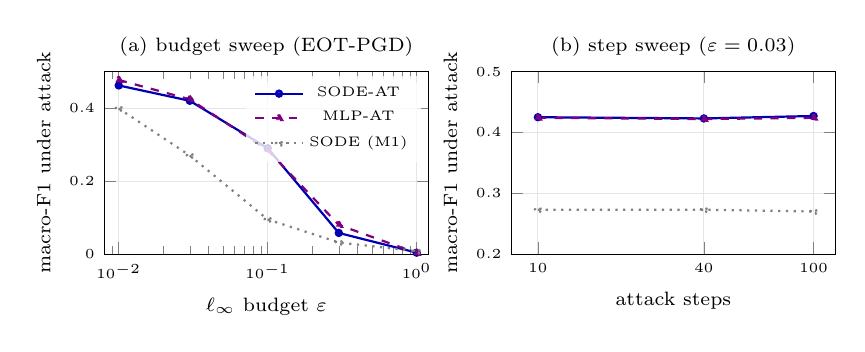
\begin{tikzpicture}
\begin{axis}[name=l, width=0.47\linewidth, height=3.9cm, xmode=log,
  xlabel={$\ell_\infty$ budget $\varepsilon$}, ylabel={macro-F1 under attack},
  xmin=0.008, xmax=1.2, ymin=0, ymax=0.5, label style={font=\scriptsize}, tick label style={font=\tiny},
  title={\scriptsize (a) budget sweep (EOT-PGD)}, title style={yshift=-4pt},
  legend style={font=\tiny, at={(0.98,0.98)}, anchor=north east, draw=none, fill=white, fill opacity=0.8, text opacity=1},
  grid=major, grid style={gray!20}]
\addplot[blue!70!black, thick, mark=*, mark size=1.1pt] coordinates {(0.01,0.462) (0.03,0.420) (0.1,0.290) (0.3,0.058) (1,0.004)};
\addplot[violet, thick, dashed, mark=triangle*, mark size=1.3pt] coordinates {(0.01,0.477) (0.03,0.424) (0.1,0.285) (0.3,0.080) (1,0.003)};
\addplot[gray, thick, dotted, mark=o, mark size=1.1pt] coordinates {(0.01,0.399) (0.03,0.270) (0.1,0.095) (0.3,0.032) (1,0.008)};
\legend{SODE-AT, MLP-AT, SODE (M1)}
\end{axis}
\begin{axis}[at={(l.east)}, anchor=west, xshift=1.05cm, width=0.47\linewidth, height=3.9cm, xmode=log,
  xlabel={attack steps}, ylabel={macro-F1 under attack},
  xmin=8, xmax=120, ymin=0.2, ymax=0.5, xtick={10,40,100}, xticklabels={10,40,100},
  label style={font=\scriptsize}, tick label style={font=\tiny},
  title={\scriptsize (b) step sweep ($\varepsilon=0.03$)}, title style={yshift=-4pt},
  grid=major, grid style={gray!20}]
\addplot[blue!70!black, thick, mark=*, mark size=1.1pt] coordinates {(10,0.425) (40,0.423) (100,0.427)};
\addplot[violet, thick, dashed, mark=triangle*, mark size=1.3pt] coordinates {(10,0.424) (40,0.422) (100,0.424)};
\addplot[gray, thick, dotted, mark=o, mark size=1.1pt] coordinates {(10,0.273) (40,0.273) (100,0.270)};
\end{axis}
\end{tikzpicture}
\caption{Gradient-masking checks on seed 0 (500 flows, EOT-PGD with fresh
paths). (a)~Macro-F1 falls steadily to near zero as the budget grows. (b)~More
attack steps never help the defender; the attack has converged.}
\label{fig:masking}
\end{figure}


\textbf{Full-strength re-attack.} On seed 0 we repeated every attack at full
strength (PGD-200 with five restarts, EOT with 32 draws, a 256-path expected
margin, Square with 5{,}000 queries, 1{,}000 flows) and certified with
$n=10{,}000$. The worst case moved by about $0.02$ or less for every model
(SODE-AT $0.427$ vs.\ $0.421$), parity with MLP-AT held ($+0.001$), and the
certified accuracy was identical to $n=2000$ (\cref{tab:checks}), so the
five-seed numbers are limited neither by attack strength nor by sample size.

\textbf{Chronological split.} Ordering each class by time (first 60\% to train,
last 20\% to test) reproduces the picture: M2 adds $0.120$ worst-case macro-F1,
SODE-AT and MLP-AT are level ($0.434$ vs.\ $0.435$), and trees fall to $0.04$
(\cref{tab:checks}).

\begin{table}[t]
\caption{Evaluation checks. Left: worst-case macro-F1 on seed 0 under the five-seed
(lite) suite on 500 flows and the full-strength suite on 1{,}000 flows. Right:
per-class chronological split, three seeds.}
\label{tab:checks}
\centering\small\setlength{\tabcolsep}{4pt}
\begin{tabular}{lcc@{\hspace{18pt}}lcc}
\toprule
\multicolumn{3}{c}{Full-strength re-attack (seed 0)} & \multicolumn{3}{c}{Chronological split (3 seeds)}\\
\cmidrule(r){1-3}\cmidrule(l){4-6}
Model & Lite & Full & Model & Clean & Worst case\\
\midrule
SODE (M1) & 0.244 & 0.240 & SODE (M1) & 0.494 & 0.309\\
SODE-AT & 0.421 & 0.427 & Neural ODE (M1) & 0.494 & 0.309\\
Neural ODE-AT & 0.422 & 0.442 & MLP (M1) & 0.492 & 0.330\\
MLP-AT & 0.419 & 0.440 & SODE-AT & 0.491 & 0.434\\
MLP (M1) & 0.279 & 0.277 & MLP-AT & 0.484 & 0.435\\
LightGBM & 0.025 & 0.031 & LightGBM & 0.602 & 0.040\\
\midrule
\multicolumn{3}{l}{Certified at $r=0.273$, $n=2000$ / $10{,}000$:} & & & \\
\multicolumn{3}{l}{\quad SODE-RS $0.602/0.602$; MLP-RS $0.554/0.554$} & & & \\
\bottomrule
\end{tabular}
\end{table}

\subsection{Realisable attacks and operating points}
\textbf{Feature-constrained attacks.} A traffic-level attacker controls only its
own packets. We therefore repeat the attacks with three restrictions in raw
feature units: only the 44 client-side statistics may change (the 31
server-side, port, protocol, flag and window features stay fixed), no feature
leaves its training range, and the 51 integer-valued features change by whole
units within the budget. The attacks are constrained PGD with restarts, EOT-PGD with fresh paths, a masked
Square search and constrained transfer. Under these limits the adversarially
trained detectors lose almost nothing (\cref{tab:constrained}): SODE-AT keeps
$0.446$ from $0.458$ on the same flows, on par with MLP-AT ($0.439$) and
ODE-AT ($0.443$). The trees still fall to $0.17$--$0.19$ from about $0.60$, so
their brittleness is not an artefact of the unconstrained threat model.

\begin{table}[t]
\caption{Macro-F1 under feature-constrained attacks (500 class-stratified test
flows per seed, five seeds, mean $\pm$ 95\% CI; fixed paths), next to the
unconstrained worst case of \cref{tab:main}.}
\label{tab:constrained}
\centering\footnotesize
\setlength{\tabcolsep}{4pt}
\begin{tabular}{lccc}
\toprule
Model & Clean (same flows) & Unconstrained worst case & Constrained worst case\\
\midrule
SODE-AT & 0.458\ci{.029} & 0.420\ci{.010} & \textbf{0.446}\ci{.022}\\
Neural ODE-AT & 0.456\ci{.028} & 0.432\ci{.028} & 0.443\ci{.019}\\
MLP-AT & 0.456\ci{.055} & 0.424\ci{.047} & 0.439\ci{.053}\\
SODE (M1) & 0.473\ci{.016} & 0.245\ci{.017} & 0.395\ci{.017}\\
MLP (M1) & 0.472\ci{.011} & 0.267\ci{.012} & 0.400\ci{.014}\\
LightGBM / XGBoost / RF & 0.608 / 0.590 / 0.576 & 0.021 / 0.015 / 0.037 & 0.172 / 0.172 / 0.186\\
\bottomrule
\end{tabular}
\end{table}

\textbf{Conformal alarm thresholds.} Operations teams set a false-alarm budget.
We fit a temperature \citep{guo2017calibration} and a split-conformal threshold
on the benign class of the held-out calibration half. The alarm fires when
$1-p_{\mathrm{benign}}$ exceeds the conformal quantile. The budget holds on
test flows for every model and seed (false-alarm rate 0.007--0.011 at a 1\%
budget and 0.047--0.050 at 5\%). At 5\%, SODE-Guard raises an alarm on 95.6\% of
attack flows, including 79--92\% of the five small attack classes that it
rarely names correctly, and SODE-AT on 85.9\%, so robustness costs some
sensitivity at a fixed budget. Class-conditional conformal sets
\citep{sadinle2019lac} cover every class at least 80\% of the time at the 90\%
level (SODE-Guard: 87\%), with about two classes per set, whereas marginal sets
almost never cover the rarest classes (\cref{tab:alarms}).

\subsection{Generalisation to a second corpus}
\Cref{tab:generalisation} repeats the full protocol on UNSW-NB15. Every
conclusion carries over:
\begin{itemize}
\item M1 and M2 help even more (clean macro-F1 $+0.144$, worst case $+0.149$).
\item The trees again lead on clean flows (by $0.16$, driven by four small attack
families) and again collapse under attack, also when constrained.
\item The masking checks pass, and the full-strength re-attack of seed 0 agrees
within $0.03$.
\end{itemize}
On this corpus SODE-Guard is significantly ahead of the matched baselines under
attack, by about one point over MLP-AT and ODE-AT (Holm-adjusted $p=0.048$). It
also certifies more than the smoothed MLP ($+0.020$, $p=0.006$), while it is
level with the smoothed neural ODE.

\begin{table}[t]
\caption{The protocol on two corpora (five seeds each; differences are paired
bootstrap estimates, $^{*}$ Holm-adjusted $p<0.05$). Worst cases use fixed paths;
certified accuracy is at $\ell_2$ radius $0.273$ on class-stratified flows.}
\label{tab:generalisation}
\centering\footnotesize
\setlength{\tabcolsep}{4pt}
\begin{tabular}{lcc}
\toprule
& ICS3D container flows & UNSW-NB15\\
\midrule
Clean macro-F1, original recipe $\to$ M1 & 0.438 $\to$ 0.495$^{*}$ & 0.508 $\to$ 0.652$^{*}$\\
Worst case, SODE (M1) $\to$ SODE-AT (M2) & 0.245 $\to$ 0.420$^{*}$ & 0.402 $\to$ 0.545$^{*}$\\
SODE-AT $-$ MLP-AT / $-$ ODE-AT, worst case & $-0.001$ / $-0.005$ & $+0.011^{*}$ / $+0.010^{*}$\\
SODE-RS certified accuracy & 0.576 & 0.453\\
SODE-RS $-$ MLP-RS / $-$ ODE-RS, certified & $+0.006$ / $-0.003$ & $+0.020^{*}$ / $+0.002$\\
Trees: clean / worst case & 0.61--0.62 / 0.02--0.04 & 0.80--0.82 / 0.04--0.11\\
Trees: constrained worst case & 0.17--0.19 & 0.05--0.11\\
SODE-AT, constrained worst case & 0.446 & 0.571\\
SODE alarms: test FAR at 1\% / 5\% budget & 0.009 / 0.049 & 0.005 / 0.055\\
\bottomrule
\end{tabular}
\end{table}

%% ==================================================================
\section{Discussion and outlook}\label{sec:disc}
%% ==================================================================
\textbf{What the results establish.} A neural SDE detector can be trained to be
accurate on rare attacks, robust to adaptive attackers and certifiably stable,
and each property comes from a module that is cheap to add: M1 costs nothing at
inference, M2 about twice a clean training step, and M3 reuses the noise the
detector already samples. The recipe transfers unchanged to an MLP and a neural
ODE, which makes it a practical default for robust flow classifiers, and the
evaluation protocol separates real robustness from evaluation artefacts.

\textbf{Practical use.} For an operations team the recipe maps onto a simple
pipeline: train with M1 and M2, deploy the eight-path predictor at line rate,
set the alarm threshold for the false-alarm budget with the conformal rule
above, and run the certificate of \cref{prop:smooth} as an offline audit on
sampled traffic or on flows that trigger an alarm. Because the certificate reuses the
detector's own randomness, the audited model and the deployed model are the
same network. For researchers, the released driver reproduces every number in
this paper with a single command, and new detectors can be dropped into the
same attacks, certificates and statistics.

\textbf{Directions we are pursuing.}
(i)~\emph{Rare classes.} The Node-RED remote-code-execution and container-escape
stages share the network footprint of the Node-RED reconnaissance stage, so they
are detected as attacks but rarely named; flow-sequence context and per-host
aggregation are the natural next step.
(ii)~\emph{Packet-level evaluation.} Our constrained attacks keep feature vectors
realisable; replaying perturbed traffic will measure robustness end to end
\citep{simonetto2024tabularbench}.
(iii)~\emph{Anisotropic certificates.} Feature-adaptive noise as in BARS and MARS
\citep{wang2023bars,huang2025mars} fits the noise prefix of M3 directly.
(iv)~\emph{More data.} Further corpora (Edge-IIoT, CSE-CIC-IDS2018, CIC-IoT-2023)
and cross-dataset transfer will extend the generalisation study.

%% ==================================================================
\section{Conclusion}\label{sec:conc}
%% ==================================================================
We presented SODE-Guard, a neural SDE intrusion detector, with a recipe of
three modules and a protocol for measuring it. We proved that randomised
smoothing remains sound when the base classifier is itself random, so the
detector is certified with its own Brownian paths, and we kept a deterministic
Lipschitz certificate for the discretised SDE. On the ICS3D container flows,
over five seeds and eight adaptive attacks, the recipe raises clean macro-F1 by $0.057$, worst-case
macro-F1 by $0.174$ and certified accuracy to $0.576$ at $\ell_2$ radius $0.273$
($0.877$ on the test class mix), on par with the strongest robust baselines and
far above gradient-boosted trees under attack, including attacks restricted to
realisable traffic changes, and its conformal alarms meet the chosen
false-alarm budget. The conclusions carry over to UNSW-NB15, where SODE-Guard is
also significantly ahead of the matched MLP. SODE-Guard and its open protocol
give practitioners a ready path to intrusion detectors that are robust by
measurement and certified by construction, and give researchers a reproducible
benchmark on which the next generation of robust, uncertainty-aware detectors
can be built and compared.

\section*{Reproducibility statement}
Architectures and hyper-parameters are in \cref{sec:model} and \cref{app:hyper};
complete proofs are in \cref{app:proofs}. The anonymised repository (\anonrepo)
contains the model, the three modules, the certifiers, every attack, the data
preparation with deduplication, the split protocols, a resumable multi-seed
driver, a Colab notebook, and the per-seed result files and summaries behind
every table and figure.

\section*{Ethics statement}
This work is defensive and aims to make intrusion detectors harder to evade. All
attacks are standard and public, and the data contain flow statistics only, with
no payloads or personal identifiers. Certificates cover the stated threat model;
a detector should be one layer of a defence in depth.

\section*{AI use statement}
%% AUTHORS: edit so that every sentence is true for this submission.
We used large-language-model assistants to copy-edit the manuscript, to draft
parts of the exposition and proofs, which the authors checked line by line, and
to write parts of the released code, which the authors tested. All results come
from the authors' own training and evaluation runs, and every citation was
checked against its source.

\bibliography{sode_guard_iclr2027}
\bibliographystyle{iclr2027_conference}

\newpage
\appendix

%% ==================================================================
\section{Proofs}\label{app:proofs}
%% ==================================================================
\paragraph{Proof of \cref{prop:smooth}.} For each class $c$ let
$u_c(z)=\Prob_\omega[\hat y(z;\omega)=c]$. Since $\omega$ is independent of $z$
and of $\epsilon$, Fubini's theorem gives
$p_c(x)=\Exp_\epsilon[u_c(x+\sigma\epsilon)]$, the convolution of the
$[0,1]$-valued function $u_c$ with $\mathcal N(0,\sigma^2I)$. By Lemma~2 of
\citet{salman2019smoothadv}, $x\mapsto\sigma\Phi^{-1}(p_c(x))$ is 1-Lipschitz in
$\ell_2$. Hence for $\|\delta\|_2<\sigma\Phi^{-1}(\underline p_A)$,
$\Phi^{-1}(p_{c_A}(x+\delta))\ge\Phi^{-1}(\underline p_A)-\|\delta\|_2/\sigma>0$,
that is $p_{c_A}(x+\delta)>\tfrac12$. Because $\sum_cp_c=1$, every other class has
$p_c(x+\delta)<\tfrac12$, so $G(x+\delta)=c_A$. For the estimate, the pairs
$(\epsilon_i,\omega_i)$, $i=1,\dots,n$, are independent and identically
distributed, so the indicators $\mathbb 1[\hat y(x+\sigma\epsilon_i;\omega_i)=c_A]$
are independent Bernoulli$(p_{c_A}(x))$ variables, and the one-sided
Clopper--Pearson bound \citep{clopper1934} satisfies
$\Prob[p_{c_A}(x)\ge\underline p_A]\ge1-\alpha$. The class $c_A$ is chosen from
$n_0$ separate draws, so it is fixed given the estimation sample. Finally, the
pure-diffusion prefix $dZ_s=\sigma\,dB_s$, $Z_0=x$, has $Z_1=x+\sigma B_1$ with
$B_1\sim\mathcal N(0,I_p)$, which is the input noise above. \hfill$\square$

\paragraph{Proof of \cref{lem:ms}.} Let $D_k=Y_k-X_k$. The constant diffusion
floor cancels, so $D_{k+1}=D_k+\Delta f_k\Delta t+\Delta g_k\Delta W_k$ with
$\Delta f_k=f_\theta(Y_k,t_k)-f_\theta(X_k,t_k)$ and
$\Delta g_k=g_\theta(Y_k,t_k)-g_\theta(X_k,t_k)$. As $\Delta W_k$ is independent
of $(X_k,Y_k)$ with mean zero and covariance $\Delta t I_m$,
$\Exp[\|D_{k+1}\|^2\mid X_k,Y_k]=\|D_k+\Delta f_k\Delta t\|^2+\Delta t\|\Delta g_k\|_F^2
\le((1+K_f\Delta t)^2+K_g^2\Delta t)\|D_k\|^2$. Iterating $n=T/\Delta t$ times with
$1+u\le e^u$ and $\|D_0\|\le L_h\|\delta\|$ gives the claim. \hfill$\square$

\paragraph{Proof of \cref{thm:mean-cert}.} Couple both expectations through the
same increments. $P_B$ is non-expansive and $\psi$ is affine with $\|W_\psi\|$,
so by Jensen, Cauchy--Schwarz and \cref{lem:ms},
$\|F^B(x+\delta)-F^B(x)\|\le\|W_\psi\|(\Exp\|Y_n-X_n\|^2)^{1/2}\le L\|\delta\|$.
Each logit difference is $\sqrt2L$-Lipschitz, so a margin $M(x)$ cannot be closed
within radius $M(x)/(\sqrt2L)$. \hfill$\square$

\begin{corollary}[Monte-Carlo certification]\label{cor:mc}
Choose $\hat y$ from $n_0$ paths. From $n_{\mathrm c}$ further paths compute the
pairwise margins $Z^{(i)}_k=(e_{\hat y}-e_k)^\tr P_B(\psi(X^{(i)}_n))$, their
means $\hat M_k$ and empirical-Bernstein widths $t_k$ \citep{maurer2009bernstein}
at level $\alpha/(K-1)$. With probability at least $1-\alpha$, if
$\underline M=\min_{k\ne\hat y}(\hat M_k-t_k)>0$, then $\hat y=\argmax F^B(x)$ and
$\underline M/(\sqrt2L)$ is a certified radius.
\end{corollary}
\emph{Proof.} Each $Z^{(i)}_k$ lies in $[-\sqrt2B,\sqrt2B]$; Theorem~4 of
\citet{maurer2009bernstein} and a union bound over the $K-1$ competitors give
$M(x)\ge\underline M$ with probability $1-\alpha$, and \cref{thm:mean-cert}
applies. \hfill$\square$

\begin{proposition}[Path-wise decision-flip bound]\label{prop:flip}
For a fixed class $k^\star$, a perturbation $\delta$ chosen independently of the
noise and the path margin $G(x)=\psi^{(k^\star)}(X_n)-\max_{k\ne k^\star}\psi^{(k)}(X_n)$,
for every $\beta>0$,
$\Prob[\argmax_k\psi^{(k)}(Y_n)\ne k^\star]\le\Prob[G(x)\le\beta]+2L^2\|\delta\|_2^2/\beta^2$.
\end{proposition}
\emph{Proof.} $|G(x+\delta)-G(x)|\le\sqrt2\|W_\psi\|\|Y_n-X_n\|$, so a flip needs
$G(x)\le\beta$ or $\sqrt2\|W_\psi\|\|Y_n-X_n\|\ge\beta$; Markov's inequality on the
square and \cref{lem:ms} bound the second event. \hfill$\square$



%% ==================================================================
\section{Additional results}\label{app:tables}
%% ==================================================================
\begin{algorithm}[h]
\caption{\textsc{CertifySmoothed}$(x)$ for the stochastic detector}
\label{alg:certify}
\begin{algorithmic}[1]
\REQUIRE flow $x$; noise level $\sigma$; $n_0$, $n$, $\alpha$; deployed predictor \eqref{eq:predictor} with fresh paths on every call
\STATE draw $n_0$ pairs $(\epsilon_i,\omega_i)$; $c_A\leftarrow$ most frequent $\hat y(x+\sigma\epsilon_i;\omega_i)$ \hfill\COMMENT{selection}
\STATE draw $n$ new pairs; $k\leftarrow\#\{i:\hat y(x+\sigma\epsilon_i;\omega_i)=c_A\}$ \hfill\COMMENT{estimation}
\STATE $\underline p_A\leftarrow$ one-sided Clopper--Pearson lower bound of $k/n$ at level $1-\alpha$
\IF{$\underline p_A>\tfrac12$} \RETURN $(c_A,\ \sigma\Phi^{-1}(\underline p_A))$ \ELSE \RETURN \textsc{abstain} \ENDIF
\end{algorithmic}
\end{algorithm}

\begin{table}[h]
\caption{Macro-F1 of SODE-AT under each attack (mean of five seeds), scored with
fixed and fresh paths; the worst case is taken per flow over all attacks.}
\label{tab:attacks}
\centering\small
\begin{tabular}{lcc}
\toprule
Attack & Fixed paths & Fresh paths\\
\midrule
PGD-40 & 0.427 & 0.424\\
PGD-100, two restarts & 0.427 & 0.434\\
APGD-CE, EOT & 0.427 & 0.428\\
APGD-DLR, EOT & 0.423 & 0.423\\
EOT-PGD-50, eight draws & 0.427 & 0.428\\
Expected margin, 64 paths & 0.422 & 0.423\\
Square, 1{,}000 queries & 0.447 & 0.451\\
Transfer from MLP / MLP-AT & 0.441 / 0.436 & 0.436 / 0.437\\
\midrule
Worst case over all attacks & 0.420 & 0.412\\
\bottomrule
\end{tabular}
\end{table}

\begin{table}[h]
\caption{Operating points on ICS3D, fitted on the calibration half and measured on
the test split (five seeds). ECE before and after temperature scaling;
class-conditional conformal sets at the 90\% level (coverage, lowest per-class
coverage, mean set size; marginal sets reach the same overall coverage but a
lowest per-class coverage near zero); conformal false-alarm thresholds with the
benign class (label 0): test false-alarm rate (FAR) and detection rate.}
\label{tab:alarms}
\centering\footnotesize
\setlength{\tabcolsep}{3.5pt}
\begin{tabular}{lcccc}
\toprule
Model & ECE & Class-conditional sets, 90\% & FAR / detection, 1\% & FAR / detection, 5\%\\
\midrule
SODE (M1) & 0.063 $\to$ 0.032 & 0.897 / 0.867 / 2.05 & 0.009 / 0.666 & 0.049 / 0.956\\
SODE-AT & 0.137 $\to$ 0.101 & 0.898 / 0.848 / 2.10 & 0.009 / 0.493 & 0.049 / 0.859\\
Neural ODE-AT & 0.122 $\to$ 0.093 & 0.898 / 0.858 / 2.10 & 0.009 / 0.485 & 0.050 / 0.872\\
MLP-AT & 0.119 $\to$ 0.094 & 0.899 / 0.835 / 2.09 & 0.009 / 0.498 & 0.048 / 0.872\\
LightGBM & 0.010 $\to$ 0.006 & 0.898 / 0.834 / 1.48 & 0.007 / 0.894 & 0.050 / 0.999\\
XGBoost & 0.012 $\to$ 0.006 & 0.899 / 0.804 / 1.44 & 0.007 / 0.900 & 0.050 / 0.999\\
Random forest & 0.008 $\to$ 0.024 & 0.903 / 0.869 / 4.39 & 0.008 / 0.881 & 0.049 / 0.999\\
\bottomrule
\end{tabular}
\end{table}


%% ==================================================================




\begin{table}[h]
\caption{Per-class clean F1 (mean of five seeds). Classes of the ICS3D container
flows (label codes 0, 1, 2, 11, 8, 6, 3, 4, 7; NR: Node-RED); flows per class
after deduplication in parentheses.}
\label{tab:perclass}
\centering\scriptsize
\setlength{\tabcolsep}{2.6pt}
\begin{tabular}{lccccccccc}
\toprule
Model & Benign & \shortstack{CVE-\\20-13379} & \shortstack{NR\\recon} & \shortstack{Nuclei\\scan} & \shortstack{CVE-\\21-25741} & \shortstack{CVE-\\19-20933} & \shortstack{NR\\RCE} & \shortstack{NR\\escape} & \shortstack{CVE-\\21-30465}\\
 & {\scriptsize(19{,}738)} & {\scriptsize(18{,}872)} & {\scriptsize(19{,}878)} & {\scriptsize(8{,}696)} & {\scriptsize(803)} & {\scriptsize(189)} & {\scriptsize(165)} & {\scriptsize(158)} & {\scriptsize(128)}\\
\midrule
SODE-base & 0.95 & 0.92 & 0.95 & 0.98 & 0.15 & 0.00 & 0.00 & 0.00 & 0.00\\
SODE (M1) & 0.96 & 0.93 & 0.96 & 0.98 & 0.29 & 0.32 & 0.02 & 0.01 & 0.00\\
SODE, square-root sampling & 0.95 & 0.93 & 0.96 & 0.98 & 0.31 & 0.38 & 0.04 & 0.00 & 0.03\\
SODE-AT & 0.94 & 0.91 & 0.95 & 0.98 & 0.20 & 0.15 & 0.04 & 0.02 & 0.01\\
MLP (M1) & 0.95 & 0.91 & 0.95 & 0.97 & 0.22 & 0.26 & 0.03 & 0.00 & 0.02\\
LightGBM & 0.98 & 0.94 & 0.97 & 0.98 & 0.44 & 0.78 & 0.13 & 0.04 & 0.30\\
XGBoost & 0.98 & 0.94 & 0.97 & 0.98 & 0.45 & 0.80 & 0.11 & 0.03 & 0.32\\
\bottomrule
\end{tabular}
\end{table}

\begin{table}[h]
\caption{Deterministic certificates on trained detectors, from the earlier
certifiable configuration (Lipschitz encoder, spectral-normalised head;
stratified 70/15/15 split without deduplication; 500 class-stratified flows;
$\alpha=10^{-3}$). $L$ is computed from exact singular values. Randomised
smoothing of an MLP is shown for reference.}
\label{tab:det-cert}
\centering\small
\begin{tabular}{lccccc}
\toprule
Certificate & $L$ & $r=0$ & $r=0.05$ & $r=0.1$ & $r=0.273$\\
\midrule
SODE-Guard, \cref{thm:mean-cert} (Monte-Carlo, \cref{cor:mc}) & 11.5 & 0.610 & 0.538 & 0.294 & 0.096\\
Neural ODE, \cref{thm:mean-cert} ($K_g=0$) & 5.1 & 0.618 & 0.608 & 0.590 & 0.280\\
Lipschitz MLP, Lipschitz margin & 1.4 & 0.618 & 0.608 & 0.590 & 0.422\\
MLP, randomised smoothing ($\sigma=0.25$) & --- & 0.636 & 0.628 & 0.628 & 0.606\\
\bottomrule
\end{tabular}
\end{table}

%% ==================================================================
\section{Data and protocol}\label{app:data}
%% ==================================================================
ICS3D \citep{anon_ics3d} combines cloud-security logs, an Edge-IIoT split and
Kubernetes/Docker container flows; we use the container flows, extracted by a
CICFlowMeter-compatible tool. Flows are read in chunks and capped at 20{,}000 per
class ($70{,}319$ flows). Identifier columns (flow ID, addresses, timestamp) and the
source port are dropped, non-numeric and mostly empty columns are removed, and
exact duplicates (325) and feature vectors with conflicting labels (1{,}250
flows) are removed before splitting. Three classes with fewer than 100 flows
after deduplication (33--48 flows) are excluded, leaving $68{,}627$ flows in 9
classes and 81 numeric columns, of which 75 have non-zero training variance.
Each seed draws a stratified 60/20/20 split ($41{,}176$ training,
$6{,}862$ selection, $6{,}863$ calibration and $13{,}726$ test flows); missing
values are filled with training medians, features are z-scored with training
statistics and clipped to $\pm10$. Attacks use 500 class-stratified test flows per
seed and certificates another 500; metrics on these subsets are also reported
reweighted to the test class mix. The chronological split orders each class by
timestamp and assigns its first 60\%, next 20\% and last 20\% to training,
validation and test.

%% ==================================================================
\section{Hyper-parameters}\label{app:hyper}
%% ==================================================================
\begin{table}[h]
\centering\small
\begin{tabularx}{\linewidth}{@{}p{0.27\linewidth}X@{}}
\toprule
Component & Setting\\
\midrule
SDE & $d=128$, $m=16$, drift and diffusion three-layer GELU perceptrons of width 256 with spectral normalisation, diffusion floor $\lambda_0=10^{-3}$, $T=1$, $\Delta t=0.05$; $M=8$ paths in training and inference\\
Optimisation (M1) & AdamW, learning rate $5\times10^{-4}$, weight decay $10^{-4}$, batch 512, cosine decay, at most 60 epochs, patience 12, gradient clipping at norm 1; logit-adjusted loss with $\tau=1$; post-hoc $\tau'$ on a grid over $[-1,2.5]$ (smoothed models: $[-4,4]$)\\
Adversarial training (M2) & N-FGSM, $\varepsilon=0.03$, noise $\mathcal U[-2\varepsilon,2\varepsilon]$, budget ramp over the first 15\% of epochs, model selection on PGD-10 macro-F1 over 1{,}000 validation flows\\
Smoothing (M3) & $\sigma=0.25$, two noisy copies, consistency weight $\lambda\in\{0,1,2\}$ (short schedule: 10), entropy weight 0.5, at least 20 epochs, patience 20, selection on the post-hoc-adjusted vote over eight noisy draws; certification $n_0=100$, $n=2000$ (check: $10{,}000$), $\alpha=10^{-3}$\\
Trees & LightGBM: 3{,}000 rounds, learning rate 0.05, 63 leaves, subsampling 0.8, early stopping after 100 rounds; XGBoost: depth 8, otherwise the same; random forest: 500 trees, balanced subsampling; balanced sample weights and post-hoc $\tau'$\\
Compute & one GPU per run (T4 or A100); mean training time per model on mixed GPUs: SODE 6.3\,min, SODE-AT 10.4\,min, SODE-RS 12.6\,min, MLP under 1\,min\\
\bottomrule
\end{tabularx}
\end{table}

\end{document}
